\documentclass[aspectratio=169]{beamer}

% Theme and colors
\usetheme{Madrid}
\usecolortheme{whale}
\definecolor{primaryblue}{RGB}{0, 102, 204}
\definecolor{accentgreen}{RGB}{0, 168, 107}
\definecolor{warnorange}{RGB}{255, 153, 0}
\setbeamercolor{structure}{fg=primaryblue}
\setbeamercolor{title}{fg=white,bg=primaryblue}
\setbeamercolor{frametitle}{fg=white,bg=primaryblue}
\setbeamercolor{block title}{bg=primaryblue,fg=white}
\setbeamercolor{block body}{bg=primaryblue!10}

% Packages
\usepackage{graphicx}
\usepackage{tikz}
\usetikzlibrary{shapes.geometric, arrows, positioning, calc, decorations.pathreplacing}
\usepackage{fontawesome5}
\usepackage{booktabs}
\usepackage{xcolor}
\usepackage{hyperref}

% Remove navigation symbols
\setbeamertemplate{navigation symbols}{}

% Smaller footer
\setbeamertemplate{footline}{
    \leavevmode%
    \hbox{%
        \begin{beamercolorbox}[wd=.5\paperwidth,ht=2ex,dp=1ex,left]{author in head/foot}%
            \hspace*{2ex}\usebeamerfont{author in head/foot}\footnotesize AI Drug Discovery
        \end{beamercolorbox}%
        \begin{beamercolorbox}[wd=.5\paperwidth,ht=2ex,dp=1ex,right]{date in head/foot}%
            \usebeamerfont{date in head/foot}\footnotesize\insertframenumber{}/\inserttotalframenumber\hspace*{2ex}
        \end{beamercolorbox}}%
    \vskip0pt%
}

% Title information
\title[AI Drug Discovery]{\textbf{AI-Powered Drug Discovery}}
\subtitle{Disease to Drug Candidates in 10 Seconds}
\author{}
\date{February 2026}
\institute{}

\begin{document}

% ============================================================================
% TITLE SLIDE
% ============================================================================
\begin{frame}
    \titlepage
\end{frame}

% ============================================================================
% SLIDE 1: PROBLEM
% ============================================================================
\begin{frame}{The Problem}
    \begin{columns}[T]
        \begin{column}{0.48\textwidth}
            \vspace{0.2cm}
            {\Large \textbf{Drug Discovery Today}}
            \vspace{0.4cm}
            
            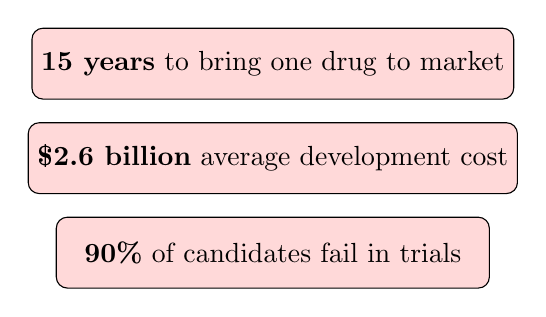
\begin{tikzpicture}
                \node[draw, fill=red!15, rounded corners, minimum width=5.5cm, minimum height=0.9cm] at (0,2.4) {\textbf{15 years} to bring one drug to market};
                \node[draw, fill=red!15, rounded corners, minimum width=5.5cm, minimum height=0.9cm] at (0,1.2) {\textbf{\$2.6 billion} average development cost};
                \node[draw, fill=red!15, rounded corners, minimum width=5.5cm, minimum height=0.9cm] at (0,0) {\textbf{90\%} of candidates fail in trials};
            \end{tikzpicture}
            
            \vspace{0.5cm}
            {\Large \textbf{The Bottleneck}}
            \vspace{0.3cm}
            
            \begin{itemize}
                \item Scientists search \textbf{4+ databases manually}
                \item Target identification takes \textbf{weeks}
                \item No unified tool connects the data
            \end{itemize}
        \end{column}
        
        \begin{column}{0.48\textwidth}
            \vspace{0.2cm}
            {\Large \textbf{Who's Affected?}}
            \vspace{0.4cm}
            
            \begin{tikzpicture}[
                box/.style={draw, rounded corners, fill=primaryblue!10, minimum width=5cm, minimum height=0.8cm, align=left}
            ]
                \node[box] at (0,3) {\faBuildingColumns\ \ \textbf{Pharma} -- Slow R\&D pipelines};
                \node[box] at (0,2) {\faFlask\ \ \textbf{Biotech} -- Limited screening resources};
                \node[box] at (0,1) {\faUniversity\ \ \textbf{Academia} -- Repetitive manual work};
                \node[box] at (0,0) {\faUserInjured\ \ \textbf{Patients} -- Years waiting for treatments};
            \end{tikzpicture}
            
            \vspace{0.5cm}
            \begin{block}{Core Problem}
                Early-stage discovery is \textbf{manual, slow,} and \textbf{fragmented} across data sources.
            \end{block}
        \end{column}
    \end{columns}
\end{frame}

% ============================================================================
% SLIDE 2: WHY NOW / WHY US
% ============================================================================
\begin{frame}{Why Now? Why Us?}
    \begin{columns}[T]
        \begin{column}{0.48\textwidth}
            \vspace{0.2cm}
            {\Large \textbf{Why Now?}}
            \vspace{0.4cm}
            
            \textbf{1. Data is Finally Available}
            \begin{itemize}
                \item AlphaFold: 200M protein structures (2022)
                \item ChEMBL: 2.4M bioactive compounds
                \item Open Targets: 12,000+ disease mappings
            \end{itemize}
            
            \vspace{0.3cm}
            \textbf{2. AI is Ready}
            \begin{itemize}
                \item BioMistral-7B: Biomedical language model
                \item Runs locally on standard hardware
                \item Async processing enables speed
            \end{itemize}
            
            \vspace{0.3cm}
            \textbf{3. Tools are Open Source}
            \begin{itemize}
                \item RDKit: Industry-standard chemistry
                \item AutoDock Vina: Free docking software
                \item All APIs are freely accessible
            \end{itemize}
        \end{column}
        
        \begin{column}{0.48\textwidth}
            \vspace{0.2cm}
            {\Large \textbf{Our Insight}}
            \vspace{0.4cm}
            
            \begin{alertblock}{First Unified Platform}
                One query connects all the pieces:
            \end{alertblock}
            
            \vspace{0.2cm}
            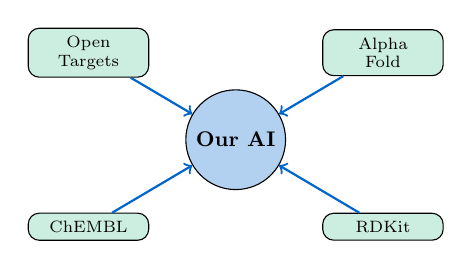
\begin{tikzpicture}[scale=0.85, transform shape]
                % Central node
                \node[draw, circle, fill=primaryblue!30, minimum size=1.4cm, font=\small\bfseries] (ai) at (0,0) {Our AI};
                
                % Surrounding nodes
                \node[draw, rounded corners, fill=accentgreen!20, minimum width=1.8cm, font=\scriptsize, align=center] (ot) at (-2.2,1.3) {Open\\Targets};
                \node[draw, rounded corners, fill=accentgreen!20, minimum width=1.8cm, font=\scriptsize, align=center] (af) at (2.2,1.3) {Alpha\\Fold};
                \node[draw, rounded corners, fill=accentgreen!20, minimum width=1.8cm, font=\scriptsize, align=center] (ch) at (-2.2,-1.3) {ChEMBL};
                \node[draw, rounded corners, fill=accentgreen!20, minimum width=1.8cm, font=\scriptsize, align=center] (rd) at (2.2,-1.3) {RDKit};
                
                % Arrows
                \draw[->, thick, primaryblue] (ot) -- (ai);
                \draw[->, thick, primaryblue] (af) -- (ai);
                \draw[->, thick, primaryblue] (ch) -- (ai);
                \draw[->, thick, primaryblue] (rd) -- (ai);
            \end{tikzpicture}
            
            \vspace{0.3cm}
            \begin{block}{Result}
                \textbf{10 seconds} instead of \textbf{weeks}\\
                Automated, ranked, AI-analyzed results
            \end{block}
        \end{column}
    \end{columns}
\end{frame}

% ============================================================================
% SLIDE 3: SOLUTION DEMO
% ============================================================================
\begin{frame}{Solution: How It Works}
    \vspace{0.2cm}
    \begin{center}
        {\Large \textbf{User Journey: Search → Results in 10 Seconds}}
    \end{center}
    
    \vspace{0.3cm}
    
    \begin{tikzpicture}[scale=0.9, transform shape]
        % Flow boxes - simplified
        \node[draw, rounded corners, fill=accentgreen!25, minimum width=2.2cm, minimum height=1.1cm, align=center, font=\small] (s1) at (0,0) {\faSearch\\\textbf{Search}};
        \node[draw, rounded corners, fill=primaryblue!15, minimum width=2.2cm, minimum height=1.1cm, align=center, font=\small] (s2) at (2.8,0) {\faBullseye\\\textbf{Targets}};
        \node[draw, rounded corners, fill=primaryblue!15, minimum width=2.2cm, minimum height=1.1cm, align=center, font=\small] (s3) at (5.6,0) {\faAtom\\\textbf{Molecules}};
        \node[draw, rounded corners, fill=primaryblue!15, minimum width=2.2cm, minimum height=1.1cm, align=center, font=\small] (s4) at (8.4,0) {\faFlask\\\textbf{Analysis}};
        \node[draw, rounded corners, fill=primaryblue!15, minimum width=2.2cm, minimum height=1.1cm, align=center, font=\small] (s5) at (11.2,0) {\faChartBar\\\textbf{Score}};
        \node[draw, rounded corners, fill=warnorange!25, minimum width=2.2cm, minimum height=1.1cm, align=center, font=\small] (s6) at (14,0) {\faList\\\textbf{Results}};
        
        % Arrows
        \draw[->, thick, primaryblue] (s1) -- (s2);
        \draw[->, thick, primaryblue] (s2) -- (s3);
        \draw[->, thick, primaryblue] (s3) -- (s4);
        \draw[->, thick, primaryblue] (s4) -- (s5);
        \draw[->, thick, primaryblue] (s5) -- (s6);
        
        % Labels below
        \node[font=\scriptsize, text=gray] at (0,-0.9) {"Alzheimer's"};
        \node[font=\scriptsize, text=gray] at (2.8,-0.9) {5 proteins};
        \node[font=\scriptsize, text=gray] at (5.6,-0.9) {100+ drugs};
        \node[font=\scriptsize, text=gray] at (8.4,-0.9) {Properties};
        \node[font=\scriptsize, text=gray] at (11.2,-0.9) {Rank 0-1};
        \node[font=\scriptsize, text=gray] at (14,-0.9) {Top 20};
        
        % Time brace
        \draw[decorate, decoration={brace, amplitude=4pt, mirror}, thick] 
            (-1,-1.4) -- (15,-1.4) node[midway, below=6pt, font=\small] {\textbf{8-10 seconds total}};
    \end{tikzpicture}
    
    \vspace{0.5cm}
    
    \begin{columns}[T]
        \begin{column}{0.32\textwidth}
            \begin{block}{\small Home Page}
                \small
                \begin{itemize}
                    \item Search box with autocomplete
                    \item Example disease queries
                    \item Clean, simple interface
                \end{itemize}
            \end{block}
        \end{column}
        
        \begin{column}{0.32\textwidth}
            \begin{block}{\small Results Page}
                \small
                \begin{itemize}
                    \item Ranked drug candidate cards
                    \item Visual score bars
                    \item Export to JSON/CSV
                \end{itemize}
            \end{block}
        \end{column}
        
        \begin{column}{0.32\textwidth}
            \begin{block}{\small Details View}
                \small
                \begin{itemize}
                    \item 2D/3D molecule structure
                    \item AI-generated analysis
                    \item Run molecular docking
                \end{itemize}
            \end{block}
        \end{column}
    \end{columns}
\end{frame}

% ============================================================================
% SLIDE 4: TECH ARCHITECTURE
% ============================================================================
\begin{frame}{Technical Architecture}
    \begin{columns}[T]
        \begin{column}{0.52\textwidth}
            \vspace{0.1cm}
            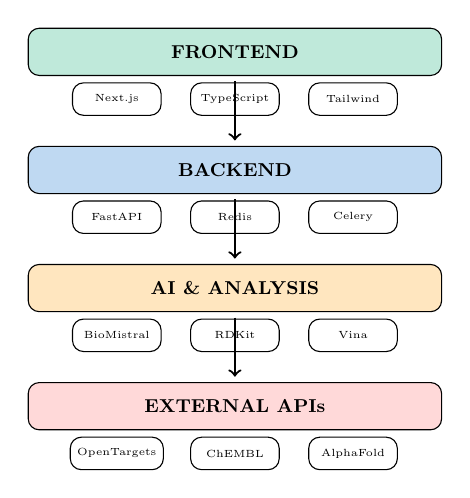
\begin{tikzpicture}[scale=0.75, transform shape]
                % Styles
                \tikzstyle{layer}=[draw, rounded corners, minimum width=7cm, minimum height=0.8cm, font=\small\bfseries]
                \tikzstyle{comp}=[draw, rounded corners, fill=white, minimum width=1.5cm, minimum height=0.55cm, font=\tiny]
                
                % Frontend
                \node[layer, fill=accentgreen!25] (fe) at (0,4.5) {FRONTEND};
                \node[comp] at (-2,3.7) {Next.js};
                \node[comp] at (0,3.7) {TypeScript};
                \node[comp] at (2,3.7) {Tailwind};
                
                % Backend
                \node[layer, fill=primaryblue!25] (be) at (0,2.5) {BACKEND};
                \node[comp] at (-2,1.7) {FastAPI};
                \node[comp] at (0,1.7) {Redis};
                \node[comp] at (2,1.7) {Celery};
                
                % AI Layer
                \node[layer, fill=warnorange!25] (ai) at (0,0.5) {AI \& ANALYSIS};
                \node[comp] at (-2,-0.3) {BioMistral};
                \node[comp] at (0,-0.3) {RDKit};
                \node[comp] at (2,-0.3) {Vina};
                
                % External
                \node[layer, fill=red!15] (ex) at (0,-1.5) {EXTERNAL APIs};
                \node[comp] at (-2,-2.3) {OpenTargets};
                \node[comp] at (0,-2.3) {ChEMBL};
                \node[comp] at (2,-2.3) {AlphaFold};
                
                % Arrows
                \draw[->, thick] (0,4) -- (0,3);
                \draw[->, thick] (0,2) -- (0,1);
                \draw[->, thick] (0,0) -- (0,-1);
            \end{tikzpicture}
        \end{column}
        
        \begin{column}{0.45\textwidth}
            \vspace{0.1cm}
            {\large \textbf{Key Components}}
            \vspace{0.3cm}
            
            \textbf{Data Sources}
            \begin{itemize}
                \small
                \item Open Targets: Disease → Proteins
                \item AlphaFold: 3D protein structures
                \item ChEMBL: Known drug molecules
            \end{itemize}
            
            \vspace{0.2cm}
            \textbf{AI Engine}
            \begin{itemize}
                \small
                \item BioMistral-7B via Ollama
                \item Generates analysis for each drug
                \item Runs locally (no cloud costs)
            \end{itemize}
            
            \vspace{0.2cm}
            \textbf{Performance}
            \vspace{0.1cm}
            
            \small
            \begin{tabular}{ll}
                \toprule
                Response time & 8-10 sec \\
                Cache hit & <100 ms \\
                Cache duration & 24 hours \\
                \bottomrule
            \end{tabular}
        \end{column}
    \end{columns}
\end{frame}

% ============================================================================
% SLIDE 5: BUSINESS MODEL
% ============================================================================
\begin{frame}{Business Model \& Go-to-Market}
    \begin{columns}[T]
        \begin{column}{0.48\textwidth}
            \vspace{0.1cm}
            {\large \textbf{Revenue Model: SaaS}}
            \vspace{0.3cm}
            
            \begin{tabular}{lll}
                \toprule
                \textbf{Tier} & \textbf{Price} & \textbf{Includes} \\
                \midrule
                Free & \$0 & 10 queries/day \\
                Pro & \$99/mo & Unlimited + API \\
                Enterprise & Custom & Docking + Support \\
                \bottomrule
            \end{tabular}
            
            \vspace{0.5cm}
            {\large \textbf{Target Customers}}
            \vspace{0.3cm}
            
            \begin{tikzpicture}
                \node[draw, rounded corners, fill=primaryblue!10, minimum width=5cm, align=left] at (0,1.5) {\faBuildingColumns\ \ Pharma R\&D teams};
                \node[draw, rounded corners, fill=primaryblue!10, minimum width=5cm, align=left] at (0,0.7) {\faFlask\ \ Biotech startups};
                \node[draw, rounded corners, fill=primaryblue!10, minimum width=5cm, align=left] at (0,-0.1) {\faUniversity\ \ University researchers};
                \node[draw, rounded corners, fill=primaryblue!10, minimum width=5cm, align=left] at (0,-0.9) {\faGraduationCap\ \ Biochemistry students};
            \end{tikzpicture}
        \end{column}
        
        \begin{column}{0.48\textwidth}
            \vspace{0.1cm}
            {\large \textbf{Go-to-Market Strategy}}
            \vspace{0.3cm}
            
            \begin{block}{\small Phase 1: Academic (Months 1-6)}
                \small
                Free tier for researchers\\
                Partner with 5 universities\\
                Build credibility with publications
            \end{block}
            
            \begin{block}{\small Phase 2: Biotech (Months 6-12)}
                \small
                Launch Pro tier\\
                API access for integrations\\
                Target 50 paying customers
            \end{block}
            
            \begin{block}{\small Phase 3: Enterprise (Year 2)}
                \small
                On-premise deployment option\\
                Custom integrations\\
                Dedicated support team
            \end{block}
        \end{column}
    \end{columns}
\end{frame}

% ============================================================================
% SLIDE 6: ROADMAP & RISKS
% ============================================================================
\begin{frame}{Roadmap \& Risks}
    \begin{columns}[T]
        \begin{column}{0.52\textwidth}
            \vspace{0.1cm}
            {\large \textbf{Development Roadmap}}
            \vspace{0.3cm}
            
            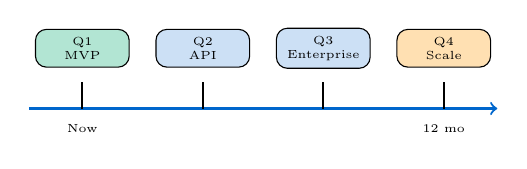
\begin{tikzpicture}[scale=0.85, transform shape]
                % Timeline arrow
                \draw[thick, ->, primaryblue] (0,0) -- (7,0);
                
                % Milestones
                \node[draw, rounded corners, fill=accentgreen!30, minimum width=1.4cm, font=\tiny, align=center] at (0.8,0.9) {Q1\\MVP};
                \draw[thick] (0.8,0) -- (0.8,0.4);
                
                \node[draw, rounded corners, fill=primaryblue!20, minimum width=1.4cm, font=\tiny, align=center] at (2.6,0.9) {Q2\\API};
                \draw[thick] (2.6,0) -- (2.6,0.4);
                
                \node[draw, rounded corners, fill=primaryblue!20, minimum width=1.4cm, font=\tiny, align=center] at (4.4,0.9) {Q3\\Enterprise};
                \draw[thick] (4.4,0) -- (4.4,0.4);
                
                \node[draw, rounded corners, fill=warnorange!30, minimum width=1.4cm, font=\tiny, align=center] at (6.2,0.9) {Q4\\Scale};
                \draw[thick] (6.2,0) -- (6.2,0.4);
                
                \node[font=\tiny] at (0.8,-0.3) {Now};
                \node[font=\tiny] at (6.2,-0.3) {12 mo};
            \end{tikzpicture}
            
            \vspace{0.4cm}
            \textbf{Milestones}
            \begin{itemize}
                \small
                \item[\faCheckCircle] Core pipeline complete
                \item[\faSpinner] Molecular docking integration
                \item[\faCircle] ADMET prediction models
                \item[\faCircle] Collaborative workspaces
            \end{itemize}
        \end{column}
        
        \begin{column}{0.45\textwidth}
            \vspace{0.1cm}
            {\large \textbf{Risks \& Mitigations}}
            \vspace{0.3cm}
            
            \small
            \textbf{Technical}
            \begin{tabular}{p{1.8cm}p{2.5cm}}
                API limits & Aggressive caching \\
                AI errors & Validation layer \\
                Scale & Cloud-ready design \\
            \end{tabular}
            
            \vspace{0.3cm}
            \textbf{Business}
            \begin{tabular}{p{1.8cm}p{2.5cm}}
                Competition & Speed to market \\
                Adoption & Free academic tier \\
            \end{tabular}
            
            \vspace{0.4cm}
            \begin{alertblock}{\small The Ask}
                \small
                \textbf{Seed: \$500K}\\
                18-month runway\\
                Hire 2 ML engineers
            \end{alertblock}
        \end{column}
    \end{columns}
\end{frame}

% ============================================================================
% CLOSING SLIDE
% ============================================================================
\begin{frame}
    \begin{center}
        \vspace{1cm}
        {\Huge\textcolor{primaryblue}{\textbf{Thank You}}}
        
        \vspace{0.8cm}
        {\Large AI-Powered Drug Discovery Platform}
        
        \vspace{0.3cm}
        {\normalsize\textcolor{gray}{From disease query to drug candidates in 10 seconds}}
        
        \vspace{1cm}
        {\large
        \faEnvelope\ \ contact@aidrugdiscovery.com\\[0.3cm]
        \faGlobe\ \ www.aidrugdiscovery.com\\[0.3cm]
        \faGithub\ \ github.com/ai-drug-discovery
        }
    \end{center}
\end{frame}

\end{document}
